%% LyX 2.3.6.1 created this file.  For more info, see http://www.lyx.org/.
%% Do not edit unless you really know what you are doing.
\documentclass[english]{article}
\usepackage[T1]{fontenc}
\usepackage[latin9]{inputenc}
\usepackage{amstext}
\usepackage{graphicx}
\usepackage{babel}
\begin{document}

\section{SIR}

SIR equations $\partial_{t}s=-\beta si$, $\partial_{t}r=\gamma i$
with the conservation law $1=s+i+r$; thus the evolution of the epidemics
plane follows the law 
\begin{equation}
\partial\ln s/\partial r=-\mathcal{R}_{0}\label{eq:main}
\end{equation}
where $\mathcal{R}_{0}=\beta/\gamma$ is the basic reproduction number.
Thus, defining $y=\ln s$, SIR epidemics have the form 
\begin{equation}
y_{E}=\ln s_{0}-\mathcal{R}_{0}\left(r-r_{0}\right)\label{eq:straight}
\end{equation}
. Notice that an epidemics end when eq.\ref{eq:straight} intersect
the boundary curve 
\begin{equation}
y_{\Omega}=\ln\left(1-r\right)\label{eq:boundary}
\end{equation}
corresponding to $r+s=1$, $i=0$. NOTE: $y_{\Omega}$ is the disease-free
equilibrium curve (also disease free set: $\Omega=\left\{ \left(s,i,r\right):i=0\land s+r=1\right\} $).
The initial state of the system at the start of an epidemics is normally
supposed to be due to a small number of infected individuals $i_{0}=\epsilon$
(i.e. $s_{0}=1-\epsilon$) that is a vanishing fraction $\epsilon\to0$
of the population; thus, a simple epidemics in the $\left(r,y\right)$
plane is a straight line starting from the point $P_{0}=\left(y=0,r=0\right)$.
Since the boundary is concave and its slope in $P_{0}$ is $\partial_{r}y_{\Omega}|_{r=0}=-1$,
the epidemics will start only if there is a non-zero intersection
of the straight line eq.\ref{eq:straight}, i.e. if $\mathcal{R}_{0}>1$.
Notice that $\mathcal{R}_{0}>1$ is also the condition for $P_{0}$to
be unstable; in fact, $\partial_{t}i>0$ for $s>\mathcal{R}_{0}^{-1}$;
since $s<1$ c.v.d. 

Notice that we must have $s_{\infty}\left(\mathcal{R}_{0},s_{0}=1\right)>\mathcal{R}_{0}^{-1}$
otherwise epidemics would not end.

This can be easily shown considering the distance among the the evolution
$y_{E}$ of the dynamics and the boundary $y_{\Omega}$. These two
curves meet at $r=0$ and $r=r_{\infty}=1-s_{\infty}$. At the beginning,
the distance will grow since $\mathcal{R}_{0}>\partial_{s}y_{\Omega}\left(r=0\right)$;
the distance will stop growing at the point $r^{*}$where the slope
of the curve is $\partial_{s}y_{\Omega}\left(r^{*}\right)=\mathcal{R}_{0}$
and will then start decreasing (remember that $y_{\Omega}$ is concave,
so $\partial_{s}y_{\Omega}$ is monotonically increasing); thus, $y_{E}$
will meet $y_{\Omega}$at a point where $\partial_{s}y_{\Omega}>\mathcal{R}_{0}$.
Notice that $\partial_{s}y_{\Omega}\left(r^{*}\right)=\mathcal{R}_{0}$
yelds $s^{*}=\mathcal{R}_{0}^{-1}$ i.e. $r^{*}=r_{\infty}$!!!

THUS, INTRODUCING LOCKDOWNS FORCES THE COMPLEX DYNAMICS TO ``LAND''
IN THE INTERVAL $\left[1-\mathcal{R}_{0}^{-1},r_{\infty}\right]$.
For $\mathcal{R}_{0}$, corresponds to $\left[0.66,0.94\right],$i.e.
from $66\%$ of the population to $94\%$ of the population.

\begin{figure}

\begin{centering}
\includegraphics[bb = 0 0 200 100, draft, type=eps]{untitled.jpg}\caption{\label{fig:1}}
\par\end{centering}
\end{figure}

NOTICE: the boundary fixpoint $y'_{\Omega}=-\mathcal{R}_{0}$ can
be solved and correspond to the boundary point $s=\mathcal{R}_{0}^{-1}$
separating $\partial_{t}i>0$ from $\partial_{t}i<0$.

POSSIBLE EXPLANATION: going to the boundaries make every time start
from $i=0$ ?????

$i_{max}$ line: $s_{max}=\mathcal{R}_{0}^{-1}$, so $0<r_{max}<1-\mathcal{R}_{0}^{-1}$,
$\ln\mathcal{R}_{0}^{-1}=\ln s_{0}-\mathcal{R}_{0}\left(r_{max}-r_{0}\right)$
\[
r_{max}=r_{0}+\mathcal{R}_{0}^{-1}\ln\left(s_{0}\mathcal{R}_{0}\right)
\]
that can be also written as 
\[
r_{max}=r_{0}+s_{max}\ln\left(\frac{s_{0}}{s_{max}}\right)
\]
.

NOTICE: when moving on the boundary I approach $s_{max}=\mathcal{R}_{0}^{-1}$,
$i_{max}$ will decrease to zero so will become ``undetectable''.
Thus, the dynamics will proceed BEYOND the boundary fixpoint, BUT
NOT MUCH.

Possible reading (???): the maximum number of infected is $s_{0}\mathcal{R}_{0}$,
so $\ln\left(s_{0}\mathcal{R}_{0}\right)$ is the number of generations
in an exponential growth and the variation in finally infected is
\# of generations / \# of new infected per infected. Or, since $\mathcal{R}_{0}^{-1}$
is the time that takes one infected individual to infect $1$ person,
it is \# of generations {*} time to infect one person (???).

\section{Fixpoint}

$s\left(r|\mathcal{R}_{0},s_{0},r_{0}\right)=s_{0}\exp\left[-\mathcal{R}_{0}\left(r-r_{0}\right)\right]$
or $r\left(s|\mathcal{R}_{0},s_{0},r_{0}\right)=r_{0}+\mathcal{R}_{0}^{-1}\ln\left(s_{0}/s\right)$;
thus the number of infected at a given initial condition $s\left(t=0\right)=s_{0}-\epsilon$,
$i\left(t=0\right)=\epsilon$, $r\left(t=0\right)=1-s_{0}$, $\epsilon\to0$
with fixed $\mathcal{R}_{0}$ is a function $i\left(s|\mathcal{R}_{0},s_{0}\right)=1-s-r\left(s|\mathcal{R}_{0},s_{0}\right)$.

$s_{\infty}$ is the intersection of the evolution $r\left(s|s_{0}\right)$
with the boundary $r=1-s$, i.e is implicitly defined by the equation
$r\left(s_{\infty}|s_{0}\right)=1-s_{\infty}$; thus it is a function
$s_{\infty}\left(\mathcal{R}_{0},s_{0}\right)$. 

Let's suppose that a $SIR$ epidemics with basic reproduction number
$\mathcal{R}_{0}>1$ is controlled via repeated lockdown strategies.
For simplicity, each lockdown starts when the number of infected reaches
a given threshold $i^{thr}$ (i.e. becomes detectable and clearly
dangerous) via non-farmacological interventions that reduce by a factor
$\alpha<1/\mathcal{R}_{0}$ the basic reproduction number, i.e. $\mathcal{R}_{0}^{lock}=\alpha\mathcal{R}_{0}<1$
. The iterative map describing such policy is:
\[
\left\{ \begin{array}{ccl}
s_{i+1}^{s} & = & s_{i}^{e}\\
s_{i+1}^{l} & : & i\left(s_{i+1}^{l}|s_{0}=s_{i+1}^{s}\right)=i^{thr}\\
s_{i+1}^{e} & = & s_{\infty}\left(\alpha\mathcal{R}_{0},s_{0}=s_{i+1}^{l}\right)
\end{array}\right.
\]
with initial condition $s_{0}^{s}=1$.

Notice that even in absence of non-farmaceutical intervention, fear
can induce social distancing leading to an effective $\mathcal{R}_{0}^{fear}<\mathcal{R}_{0}$
that would eventually lead to a fixpoint lower than $s^{\infty}$.

Notice that the ``best'' outcome of the fixpoint is $s_{max}=\mathcal{R}_{0}^{-1}$,
strictly correlated with the quantity $v_{c}=1-\mathcal{R}_{0}^{-1}$
called the critical vaccination coverage. Its interpretation is that
if at least the fraction $v_{c}$ is vaccinated, then the whole community
is protected from major outbreaks. The community is then said to have
herd immunity. NOTICE THAT THIS IS TRUE ALSO FOR STOCHASTIC MODELS.

\begin{figure}

\begin{centering}
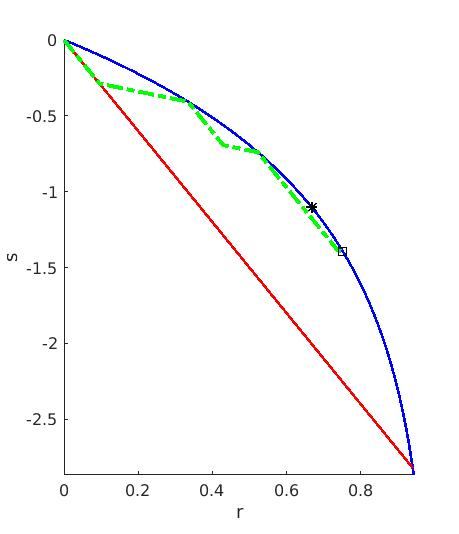
\includegraphics{untitled2}\caption{}
\par\end{centering}
\end{figure}


\section{Lockdown and stability of the boundary}

$P_{0}=\left(r_{0},s_{0}=1-r_{0}\right)$ . 

$y_{\Omega}\left(r+\delta\right)=y_{\Omega}+y'_{\Omega}\delta+\left(y'_{\Omega}\delta\right)^{2}/2+\mathcal{O}\left(\delta^{3}\right)$,
$y\left(r+\delta\right)=y-\mathcal{R}_{0}\delta$.

Solving $y(r+\delta)=y_{\Omega}\left(r+\delta\right)$ with $y(r)=y_{\Omega}\left(r\right)$
we have $y'_{\Omega}\delta+\left(y'_{\Omega}\delta\right)^{2}/2=-\mathcal{R}_{0}\delta$
i.e. $\delta=-\left(y'_{\Omega}+\mathcal{R}_{0}\right)/\left(y'_{\Omega}\right)^{2}>0$
for $\mathcal{R}_{0}>-y'_{\Omega}=\left(1-r_{0}\right)^{-1}$. 

$P_{\epsilon}=P_{0}+\left(0,-\epsilon\right)$ i.e. $y=y_{\Omega}-\epsilon$.

Solving $y(r+\delta)=y_{\Omega}\left(r+\delta\right)$ with $y(r)=y_{\Omega}\left(r\right)$
we have $\left(y'_{\Omega}\right)^{2}\delta^{2}/2+\left(y'_{\Omega}+\mathcal{R}_{0}\right)\delta-\epsilon=0$.
In the special case $y'_{\Omega}+\mathcal{R}_{0}=0$ (i.e. at the
fixpoint!!!), we have to solve just $\left(y'_{\Omega}\right)^{2}\delta^{2}/2-\epsilon=0$
so that $\delta\propto\sqrt{\epsilon}$. BEFORE the fixpoint, we are
in the case $y'_{\Omega}+\mathcal{R}_{0}>0$. Thus, the only positive
root can be

\[
\delta=\frac{-\left(y'_{\Omega}+\mathcal{R}_{0}\right)+\sqrt{\left(y'_{\Omega}+\mathcal{R}_{0}\right)^{2}+2\epsilon\left(y'_{\Omega}\right)^{2}}}{\left(y'_{\Omega}\right)^{2}}
\]

\[
\delta=\frac{y'_{\Omega}+\mathcal{R}_{0}}{\left(y'_{\Omega}\right)^{2}}\left(-1+\sqrt{1+2\epsilon\left(\frac{y'_{\Omega}}{y'_{\Omega}+\mathcal{R}_{0}}\right)^{2}}\right)
\]
. If we are far away $y'_{\Omega}+\mathcal{R}_{0}=0$, we can use
$\sqrt{1+x}\approx1+x/2$ to derive the approximation 
\[
\delta\approx\frac{\epsilon}{y'_{\Omega}+\mathcal{R}_{0}}
\]
. 

AFTER the fixpoint, we are in the case $y'_{\Omega}+\mathcal{R}_{0}<0$
so we have to solve for the \emph{least} root

\[
\delta=\frac{-\left(y'_{\Omega}+\mathcal{R}_{0}\right)-\sqrt{\left(y'_{\Omega}+\mathcal{R}_{0}\right)^{2}+2\epsilon\left(y'_{\Omega}\right)^{2}}}{\left(y'_{\Omega}\right)^{2}}
\]

\[
\delta=\frac{-\left(y'_{\Omega}+\mathcal{R}_{0}\right)}{\left(y'_{\Omega}\right)^{2}}\left(1+\sqrt{1+2\epsilon\left(\frac{y'_{\Omega}}{y'_{\Omega}+\mathcal{R}_{0}}\right)^{2}}\right)
\]
. If we are far away $y'_{\Omega}+\mathcal{R}_{0}=0$, we can use
$\sqrt{1+x}\approx1+x/2$ to derive the approximation 
\[
\delta\approx\frac{-\left(y'_{\Omega}+\mathcal{R}_{0}\right)}{\left(y'_{\Omega}\right)^{2}}\left[2+\epsilon\left(\frac{y'_{\Omega}}{y'_{\Omega}+\mathcal{R}_{0}}\right)^{2}\right]
\]
????? . It would be more reasonable to have for both sides the approx

\[
\delta\approx\left\{ \begin{array}{lcc}
\frac{\epsilon}{\left|y'_{\Omega}+\mathcal{R}_{0}\right|} & \textrm{for} & \left|y'_{\Omega}+\mathcal{R}_{0}\right|\gg\epsilon\\
\frac{\sqrt{2\epsilon}}{\left|y'_{\Omega}\right|} & \textrm{for} & \left|y'_{\Omega}+\mathcal{R}_{0}\right|\approx\epsilon
\end{array}\right.
\]
that is symmetric and nice ....

\section{SEIR}

For the $SEIR$ model 
\[
\begin{array}{lcl}
\partial_{t}S & = & -\beta SI\\
\partial_{t}E & = & \beta SI-\rho E\\
\partial_{t}I & = & \rho E-\gamma I\\
\partial_{t}R & = & \gamma I
\end{array}
\]
we still have $d\ln=-\mathcal{R}_{0}dR$ so in the $\left(y,r\right)$
plane the trajectories are straight line like in the $SIR$ model
and the boundary $y_{\Omega}(r)$ is also the same; thus, the analysis
proceeds on same ground. At difference with $SIR$, at the line $s^{*}=\mathcal{R}_{0}^{-1}$
we have the maximum of $i+e$; CHECK: the maxima of $e$ must happen
for $s>s^{*}$ (earlier in time) while the maxima of $i$ must happen
for $s<s^{*}$ (later in time).

\section{Security thresholds}

To avoid overwhelming the emergency care units of national health
services (NHSs), it is important to avoid that the number of infectious
goes beyond a given threshold $\theta$. In the $r-s$ plane, this
corresponds to the straight lines $s=\left(1-\theta\right)-r$ that
are parallel to the boundary $s=1-r$. Thus, we can define the boundary

\[
y^{\theta}=\log\left(1-\theta-r\right)
\]
. Thus, to avoid overwhelming a NHS, lockdown strategies have to constrain
the dynamic in the region $y^{\theta}\leq y\leq y^{\Omega}$. Notice
that for the $SEIR$ model this is an upper bound, since $1-s-r=i+e\leq i$.

\begin{figure}
\centering{}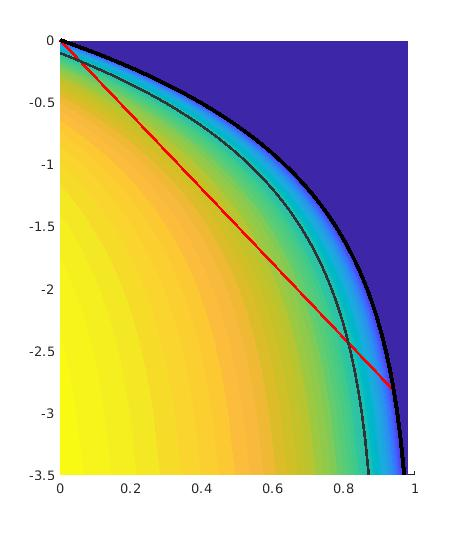
\includegraphics{untitled3}\caption{}
\end{figure}


\section{Notes}

Up to now, final size of the epidemic has taken into account 
\begin{itemize}
\item etherogeneous population
\item periods of different infectiveness
\item partial immunization by previous diseases 
\item pharmacological interventions
\end{itemize}
.... the effect of an epidemic of a pathogen inducing partial immunity
on the possibility and size of a future epidemic. In the latter case,
we prove a surprising $50\%$ law: if infection by a pathogen induces
a partial immunity reducing susceptibility by less than $50\%$, then,
whatever the value of $R_{0}>1$ before the first epidemic, a second
epidemic will occur, while if susceptibility is reduced by more than
$50\%$, then a second epidemic will only occur if $R_{0}$ is larger
than a certain critical value greater than $1$ \cite{Katriel2012size}.

Ma introduces the $SI^{n}R$ model 
\[
\begin{array}{lcl}
\partial_{t}S & = & -S\sum\beta_{i}I_{i}\\
\partial_{t}I_{1} & = & S\sum\beta_{i}I_{i}-\gamma_{1}I_{1}\\
\partial_{t}I_{i+1} & = & \gamma_{i}I_{i}-\gamma_{i+1}I_{i+1}\\
\partial_{t}R & = & \gamma_{n}I_{n}
\end{array}
\]
(note: $SEIR$ is a $SI^{2}N$ model where the $1^{st}$ stage is
not infective) and shows that latent periods do not change the final
formula for the attack ratio {[}Ma2006{]}.

Miller derives an analytical formula for the final size for an epidemics
with two infectious periods with different infectiousness \cite{Miller2012note}.

To consider behavioral response to an outbreak of a severe disease,
Brauer analyses the final size when the contact rate that decreases
in time, \cite{Brauer2019final}.

In {[}Arino2007{]}, $\mathcal{R}_{0}$ is calculated for points starting
on the disease-free set $\left(\vec{s},0,\vec{r}\right)$; also, they
show for a SARS model that includes quarantine and isolation arranged
prior to the beginning of the epidemic, that the attack ratio depends
on the control reproduction number, denoted by $\mathcal{R}_{C}$
{[}9{]} rather than the basic reproduction number $\mathcal{R}_{0}$. 

{[}9{]} A. Gumel, S. Ruan, T. Day, J. Watmough, F. Brauer, P. van
den Driessche, D. Gabrielson, C. Bowman, M.E. Alexander, S. Ardal,
J. Wu, \& B.M. Sahai, Modelling strategies for controlling SARS outbreaks,
Proc. Roy. Soc. London B 271, 2223--2232 (2004).

\bibliographystyle{plain}
\bibliography{EpidemicSize}

\end{document}
